\documentclass[a4paper,12pt,numbers=enddot]{scrartcl}

% Packages
\usepackage[utf8]{inputenc}
\usepackage[english]{babel}
\usepackage[a4paper,left=2.5cm,right=2.5cm,top=2cm,bottom=2.5cm]{geometry}
\usepackage{setspace}
\usepackage{fancyhdr}
\usepackage{cite}
\usepackage[square,numbers]{natbib}
\usepackage{graphicx}

% Settings
\bibliographystyle{dinat}
\setlength\parindent{0pt}
\pagestyle{fancy}

% Header and Footer
\fancyhead[LE,LO]{20th June 2022}
\fancyhead[RE,RO]{Exposé}
\fancyhead[CE,CO]{Group: \glqq We're not quite sure what we're doing\grqq}
\fancyfoot{}

\begin{document}

\singlespacing

\begin{Large}
\begin{center}
\textbf{Explicit Sentiment Analysis with Language Patterns about Uncertainty}
\end{center}
\end{Large}

Our goal with this project is divided into two parts. First of all we extract a dataset about semantic uncertainty from the web archive data \citep{Kiesel2018}. This dataset is then compared to Sentiment140 \citep{Sent140} to clarify how well our dataset conforms with this sentiment classification dataset. In the second part a sentiment classifier based on DistilBERT and finetuned on SST-2 \citep{DistilBert} is trained on our dataset using transfer learning. This model is benchmarked on the previous mentioned dataset to see if our dataset is suited to improve sentiment classification.
\begin{figure}[htb]
	\centering
	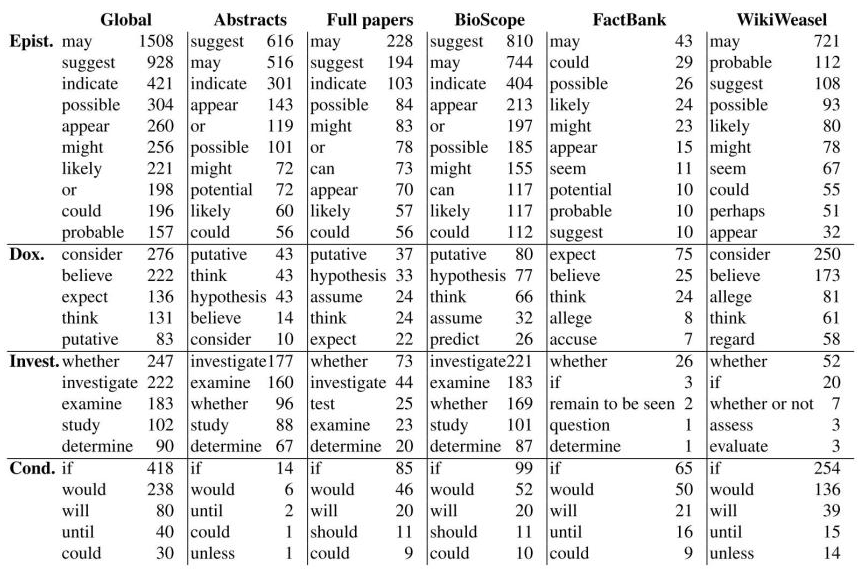
\includegraphics[scale=0.55]{language_patterns.png}
	\caption{The most frequent semantic cues in the English corpora \citep{vincze2014uncertainty}}
\end{figure}

We will use specific language patterns about uncertainty to extract samples from web archive data. An overview of the patterns can be found here \citep[p. 43]{vincze2014uncertainty}. To classify these samples into positive/negative sentiments we will mainly use GPT-3. Since we cannot fully trust results based on GPT-3 we will verify some of the labels manually. We plan to analyse our dataset based on what topics the internet is most uncertain about and how those topics changed over time using circular packing charts. After the labeling process we want to compare strong positive/negative topics of our data with those of the dataset mentioned above.
\\

In the next step we train our model. We prevent train-test leakage with the known train-validation-test split method. Furthermore we exclude all Twitter domain names from the web archive because Sentiment140 is based on statements from Twitter. The ratios of this split depends on the amount of samples we actually get in the end. We then compare our model and the baseline model with regards to the performance on Sentiment140 dataset.
\\

This leads us to the following two research questions:
\begin{itemize}
	\setlength\itemsep{-5pt}
	\item Does finetuning on uncertain statements improve sentiment classification?
	\item What are topics the internet is most uncertain about and have those topics changed over time?
\end{itemize}

The project will be split in the following three work packages:
\begin{itemize}
	\setlength\itemsep{-5pt}
	\item Dataset extraction from the web archive data
	\item Labeling, analyzing, visualizing the dataset and comparing it to Sentiment140
	\item Train a model and evaluate it on said dataset
\end{itemize}

Deliverables of the project are:
\begin{itemize}
	\setlength\itemsep{-5pt}
	\item A Dataset consisting of only uncertain statements (including datasheet)
	\item Visualizations and analysis of said dataset
	\item A DistilBERT model trained on said dataset (including model card)
\end{itemize}
\medskip

\hrule
\vspace{-2.5em}
\renewcommand{\refname}{}
\nocite{*}
\bibliography{literature}

\end{document}